\section{Experiments}


\frame
{
	\frametitle{Outdoor experiments}
		
	\begin{columns}[T]
		\column{.65\textwidth}
		\begin{itemize}
			\item New College dataset
			\item 1800 basepoints 550 m
			\item Contains gradual changes
		\end{itemize}
		\centering
		\begin{figure}[p]
			\hspace{0.5cm}
			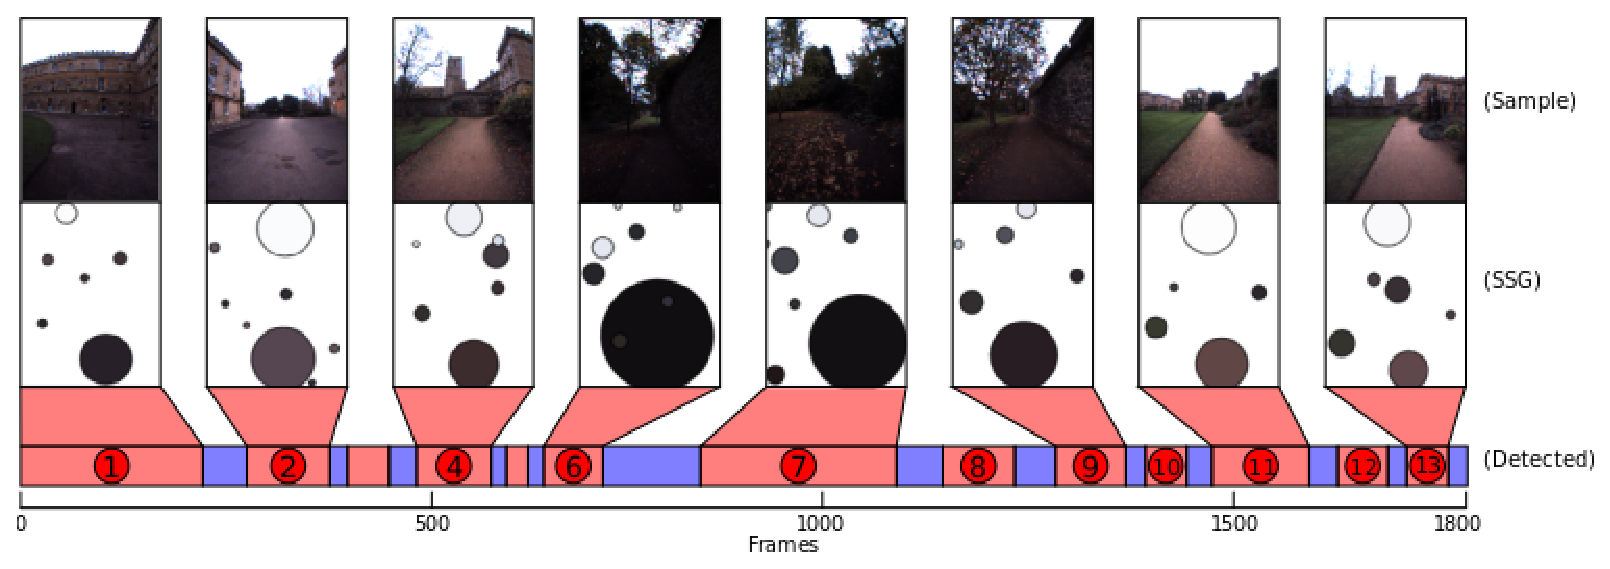
\includegraphics[width = 1\textwidth]{img/icsc/detected_places_nc}
			\label{fig:nc_ssg}
		\end{figure}

		\column{.35\textwidth}
		\centering New College Map
		\begin{figure}[p]
			\centering
			\hspace{0.5cm}
			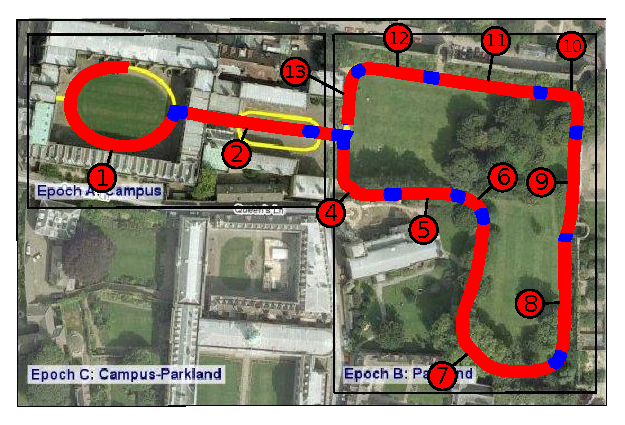
\includegraphics[width = 1.0\textwidth]{img/icsc/detected_places_nc_map}
			\label{fig:nc_map}
		\end{figure}
		

	\end{columns}		
	
}
\frame
{
	\frametitle{Indoor experiments}
	

	\begin{columns}[T]
		\column{.75\textwidth}
		
		\small
		\begin{itemize}
			\item Freiburg (Fr), Saarbrucken (Sa) and Ljubljana sites of COLD Dataset
		\end{itemize}
		\centering
		\begin{figure}[p]
			\centering
			\vspace{-0.5cm}
			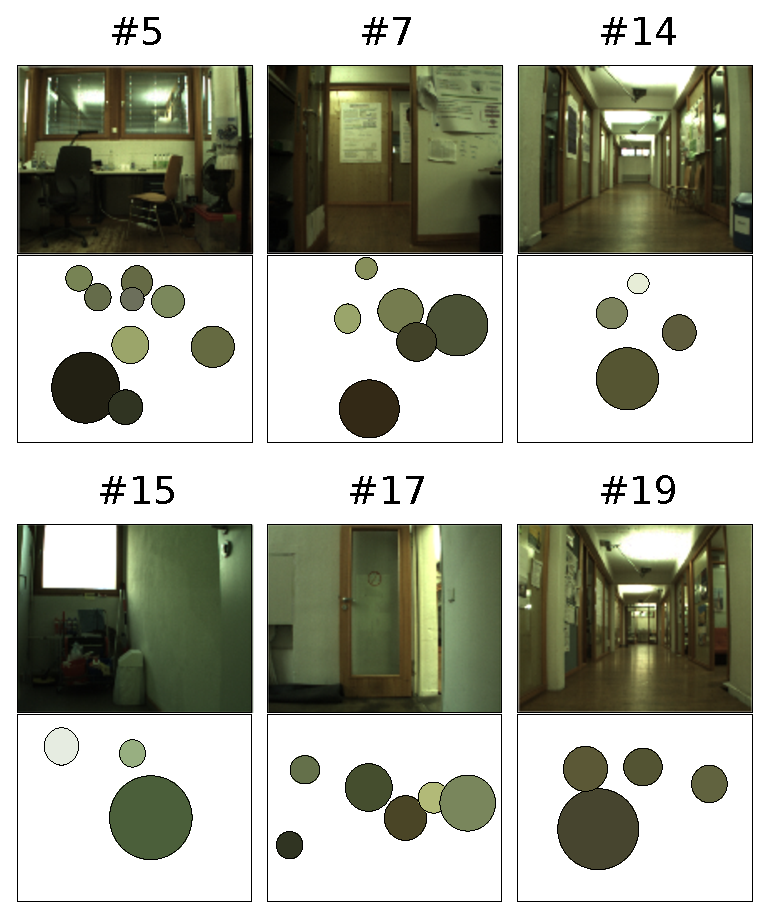
\includegraphics[width = 0.45\textwidth]{img/icsc/ssg-eval2}
			\label{fig:fr_ssg}
		\end{figure}
				
		\column{.25\textwidth}
		\begin{figure}[p]
			\centering Freiburg site
			\hspace{-0cm}
			\includegraphics[width = 1.0\textwidth]{img/icsc/detected_places_fr2_ssg}
			\label{fig:fr_map}
		\end{figure}
		

		
	\end{columns}		

}
\frame
{
	\frametitle{Comparison of Detected Places: SSG vs BD$^1$ (Bubble Descriptors) }
	
	\begin{columns}[T]
		\column{.5\textwidth}
		\small
		\centering
		SSG approach
		\vspace{-0.3cm}
		\begin{figure}[p]
			\centering
			\includegraphics[width = 0.5\textwidth]{img/master/detected_places_fr2_ssg.eps}
		\end{figure}
		\column{.5\textwidth}
		\small
		\centering
		BD approach
		\vspace{-0.3cm}
		\begin{figure}[p]
			\centering
			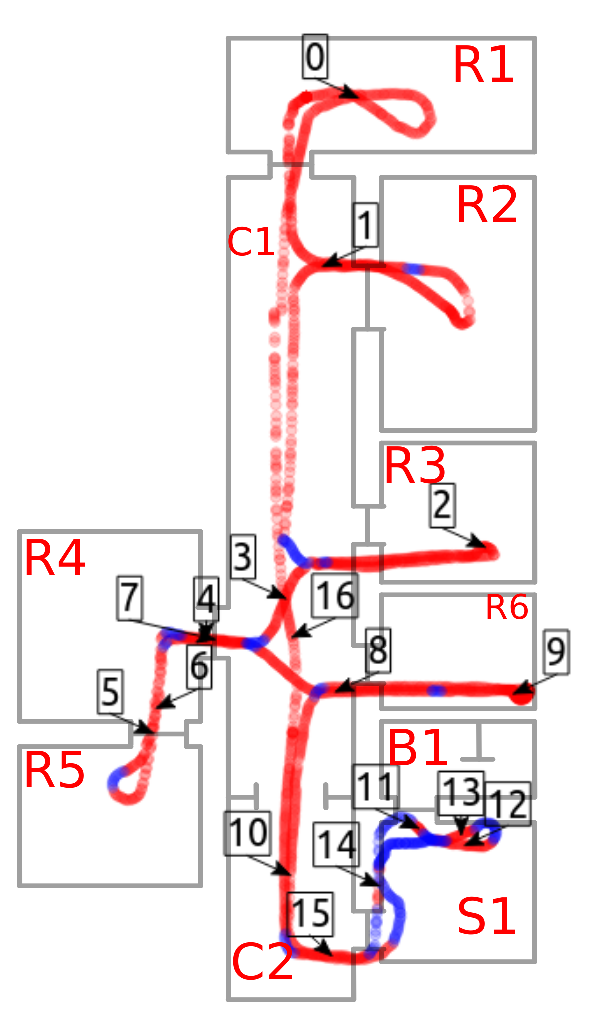
\includegraphics[width = 0.5\textwidth]{img/master/detected_places_fr2_bd.eps}
		\end{figure}
	\end{columns}
	
	\vspace*{2mm}	
	\noindent \textit{\tiny 1 - Karaoguz \& Bozma,  ICRA 2014, Autonomous Robots 2015	}
}
\frame
{
	\frametitle{VPC2009 Dataset}
	
	\begin{columns}[t,onlytextwidth]
		\hspace*{-1cm}
		
		\column{.99\textwidth}
		\vspace{-0.5cm}
		\small
		\begin{itemize}
			\item 21019 images from three different homes
			\item Challenging dateset:
			\begin{itemize}
				\item Unclear place boundaries
				\item Visual content varies
greatly with respect to the viewpoint due to small FOV
			\end{itemize}
			\item Comparison based on 43 manually annotated transition regions
			\item Criteria: Minimum \%30 overlap 
		\end{itemize}
		\centering
		\begin{tabular}{|l|l|l|l|l|}
			\hline
			Approach               & SSG  & BuS  \\ \hline
			Correct detection (\%) & 88.3 & 84.9 \\ \hline
		\end{tabular}
	\end{columns}
}
